\documentclass[portuguese]{textolivre}

% metadata
\journalname{Texto Livre}
\thevolume{17}
%\thenumber{1} % old template
\theyear{2024}
\receiveddate{\DTMdisplaydate{2024}{5}{29}{-1}}
\accepteddate{\DTMdisplaydate{2024}{7}{19}{-1}}
\publisheddate{\today}
\corrauthor{Ana Beatriz Gomes Pimenta de Carvalho}
\articledoi{10.1590/1983-3652.2024.52809}
%\articleid{NNNN} % if the article ID is not the last 5 numbers of its DOI, provide it using \articleid{} commmand 
% list of available sesscions in the journal: articles, dossier, reports, essays, reviews, interviews, editorial
\articlesessionname{articles}
\runningauthor{Carvalho}
%\editorname{Leonardo Araújo} % old template
\sectioneditorname{Daniervelin Pereira}
\layouteditorname{João Mesquita}

\title{FAB LAB e educação no Brasil: as ações de disseminação da cultura maker na educação básica e no ensino superior}
\othertitle{FAB LAB and education in Brazil: actions to disseminate the maker culture in basic and higher Education}

\author[1]{Ana Beatriz Gomes Pimenta de Carvalho ~\orcid{0000-0002-2572-7383}\thanks{Email: \href{mailto:anabeatriz.carvalho@ufpe.br}{anabeatriz.carvalho@ufpe.br}}}
\affil[1]{Universidade Federal de Pernambuco, Programa de Pós-Graduação em Educação Matemática e Tecnológica, Recife, PE, Brasil.}

\addbibresource{article.bib}

\begin{document}
\maketitle
\begin{polyabstract}
\begin{abstract}
A proposta da presente pesquisa é analisar as estratégias e ações de disseminação da cultura maker no campo da educação promovidas pelos Laboratórios de Fabricação Digital (FAB LAB) no Brasil, considerando os elementos para o desenvolvimento do letramento digital e científico, bem como os aspectos relacionados à diversidade e ao incentivo ao STEAM. A metodologia proposta foi orientada pelos princípios da pesquisa qualitativa, documental, com fundamentação teórica no campo dos Estudos Culturais. Foram analisados os documentos de quarenta e dois FAB LAB brasileiros que indicaram em seus documentos ações no campo da Educação. Os resultados indicam que existe uma grande diversidade de abordagens e ações pedagógicas nesses espaços, uso do \textit{maker} como uma ação de marketing em instituições públicas e privadas, limitações das ações efetivas direcionadas para a Educação Básica e Ensino Superior, poucas ações de diversidade e incentivo ao STEAM e letramento científico. A princípio, a diversidade de metodologias e teorias que perpassam o uso dos elementos da cultura \textit{maker} na Educação parece um ajuste necessário para o desenvolvimento de propostas integradas ao currículo e as concepções de aprendizagem adotadas em algumas instituições, mas na prática surgem como uma bricolagem com elementos conflitantes que comprometem os resultados das propostas. Apesar das limitações encontradas, a existência de propostas de espaço \textit{maker} comprometidos com a disseminação e consolidação da cultura \textit{maker} na Educação mostra que é possível articular ações efetivas com excelentes resultados.

\keywords{Cultura \textit{maker} \sep FAB LAB \sep Educação básica \sep Ensino superior \sep STEAM}
\end{abstract}

\begin{english}
\begin{abstract}
The purpose of the present research is to analyze the strategies and actions for disseminating the maker culture in the field of education, promoted by the Digital Fabrication Laboratories (FAB LAB) in Brazil, considering the elements for the development of digital and scientific literacy, as well as aspects related to diversity and the promotion of STEAM. The proposed methodology was guided by the principles of qualitative research and documentary analysis, with a theoretical foundation in the field of Cultural Studies. Documents from forty-two Brazilian FAB LABs that indicated educational actions in their documentation were analyzed. The results indicate a great diversity of approaches and pedagogical actions in these spaces, the use of maker culture as a marketing strategy in public and private institutions, limitations of effective actions directed towards Basic and Higher Education, and few actions related to diversity, promotion of STEAM, and scientific literacy. Initially, the diversity of methodologies and theories that permeate the use of maker culture elements in education seems like a necessary adjustment for the development of curriculum-integrated proposals and the learning concepts adopted by some institutions. However, in practice, they emerge as a bricolage with conflicting elements that compromise the outcomes of the proposals. Despite the limitations encountered, the existence of maker space proposals committed to the dissemination and consolidation of maker culture in education demonstrates that it is possible to articulate effective actions with excellent results.

\keywords{Maker culture \sep FAB LAB \sep Basic education \sep Higher education \sep STEAM}
\end{abstract}
\end{english}
\end{polyabstract}

\section{Introdução}
Para que a educação também acompanhe o processo de modernização ou inovação tecnológica, na perspectiva da construção do letramento digital e letramento científico, entendemos que a questão cultural é o cerne de qualquer discussão sobre as mudanças paradigmáticas mediadas pelo uso das tecnologias, e precisa ser pensada em novos contextos e perspectivas. O processo de apropriação das tecnologias digitais nas escolas é fundamental para a construção de uma relação crítica com as diversas tecnologias disponíveis, tornando-se um contraponto ao comportamento passivo e consumista que produz sujeitos vulneráveis ao processo de monitoramento, manipulação e sedução do \textit{marketing} das empresas.

A abordagem para o uso das tecnologias digitais no contexto educacional precisa considerar os elementos que contemplem a complexidade do ecossistema digital, composto por redes de Tecnologia de Informação e Comunicação, redes sociais e redes de conhecimento. A compreensão da dinâmica dessas redes e a diversidade de interesses que disputam relevância nesse ecossistema são fundamentais para o desenvolvimento de um letramento digital crítico, que propõe um usuário como participante ativo desse sistema, e não como um consumidor passivo e suscetível ao controle das grandes corporações tecnológicas, as chamadas \textit{big tech} \cite{silveira_como_2023}.

O enfrentamento das questões relacionadas à inclusão digital nas escolas e à incorporação de tecnologias digitais no currículo esteve presente no movimento do software livre, em programas governamentais de compra de equipamentos com software livre e na própria BNCC \cite{brasil_base_2018}, que menciona a cidadania digital e, mais recentemente, com a publicação de seu complemento, a programação como um diferencial para formar cidadãos preparados para uma sociedade conectada \cite{brasil_parecer_2022}.

Para abordar as questões relacionadas com a tecnologia e a aprendizagem, temos a perspectiva de construção do letramento digital e letramento científico como base da relação dos alunos com o conhecimento informacional e científico \cite{carvalho_divulgacao_2023}. É possível identificar uma preocupação crescente com o ensino de programação cada vez mais cedo e a necessidade de se estruturar as bases do pensamento científico desde as séries iniciais. No contexto atual, pode parecer absurdo que alguns grupos defendam o ``terraplanismo'' ou o movimento antivacina, mas o assunto é muito sério e requer um posicionamento científico firme e ações concretas na formação escolar de crianças e adolescentes, principalmente em relação ao volume de informações que circula atualmente em diversas mídias digitais.

A UNESCO sinalizou a importância dos letramentos midiáticos ao lançar há mais de 10 anos, em 2013, o documento \textit{Alfabetização midiática e informacional: currículo para a formação de professores}, para orientar os professores sobre a importância do tema como ``um pré-requisito importante para promover o acesso igualitário à informação e ao conhecimento e aos sistemas de mídia e informação livres, independentes e plurais'' \cite[p.~5]{wilson_alfabetizacao_2013}.

Para esta pesquisa, compreendemos o letramento digital como prática social culturalmente constituída que inclui não apenas o uso instrumental das tecnologias digitais, mas principalmente o seu processo de apropriação tecnológica. Como prática social, o letramento digital deve ser desenvolvido no contexto de formação de crianças e adolescentes, considerando que vivemos em uma sociedade informacional e a escola não pode existir dentro de uma bolha analógica em uma sociedade  predominantemente digital. Já o desenvolvimento do letramento científico parece algo inerente ao processo de formação, se considerarmos que a escola no Brasil é laica e deve ser um espaço de reprodução do conhecimento científico.

Entretanto, a construção do letramento científico envolve outros elementos que não se restringem ao processo de transmissão de conteúdo. Nesta pesquisa, letramento científico é compreendido como as competências e habilidades necessárias para o domínio e compreensão de termos científicos, que possibilitem a sua utilização adequada. Para Teixeira (2007), ``o cidadão letrado cientificamente lê, escreve e cultiva práticas sociais envolvidas com a ciência, ou seja, faz parte da cultura científica'' \cite[p.~27]{teixeira_categorizacao_2007}.

As diferentes abordagens para o uso de tecnologias digitais em sala de aula incluem robótica, metodologias ativas, PBL (aprendizagem baseada em problemas), gamificação, projetos de trabalho e, mais recentemente, elementos da cultura \textit{maker}. A proposta do movimento \textit{maker} é revolucionar a forma como produzimos e consumimos por meio de novas formas de apropriação do conhecimento derivadas do DIY (\textit{Do it Yourself}) ou ``faça você mesmo''. A cultura \textit{maker} compreende o uso de elementos da robótica, software livre, impressoras 3D, cortadoras a laser, entre outros. Mais importante do que os equipamentos e softwares, os princípios da cultura \textit{maker}, como colaboração, compartilhamento e democratização do acesso as tecnologias digitais, são materializados no desenvolvimento de projetos e resoluções de problemas que se constituem como importantes elementos para a construção do letramento científico na Educação Básica.

No Brasil, identificamos previamente várias ações que utilizam os elementos da cultura \textit{maker} na Educação e encontramos várias iniciativas em instituições públicas e financiadas por empresas nacionais e grandes corporações internacionais, por meio de suas fundações. Temos alguns exemplos, como o Projeto Mão na Massa (Instituto Porvir/Inspirare), Instituto Euvaldo Lodi, Fundação Lemann, Universidade do Vale do Itajaí, Universidade de São Paulo etc. A rede FAB LAB gerencia a implementação de FAB LAB nas principais cidades, com foco no empreendedorismo, embora alguns projetos façam parcerias com escolas e sistemas públicos de educação para a formação de professores e alunos.

Assim, o objetivo deste artigo é analisar as estratégias e ações de disseminação da cultura maker no campo da educação promovidas pelos Laboratórios de Fabricação Digital (FAB LAB) no Brasil, considerando os elementos para o desenvolvimento do letramento digital e científico, bem como os aspectos relacionados à diversidade e ao incentivo ao STEAM\footnote{STEM é a sigla em inglês utilizada para denominar as áreas do conhecimento de Science (Ciência), Tecnology (Tecnologia), Engineering (Engenharia) e Mathematics (Matemática) e STEAM, adotada nessa pesquisa, é a sigla para Ciência, Tecnologia, Engenharia, Artes e Matemática.}.

\section{Movimento \textit{maker} e a Educação}\label{sec-normas}
O movimento \textit{Do It Yourself} (DIY) surgiu como contraponto ao modelo de produção massificado e em larga escala que prevaleceu até a década de 1970, padronizando o consumo com grandes empresas, estabelecendo as demandas da sociedade. A proposta do DIY em 1950 era que as pessoas poderiam produzir pequenos objetos, resolver problemas domésticos criando soluções e realizando pequenos consertos. A partir da década de 1970, o DIY foi apropriado pelo movimento de contracultura, que resistia à lógica capitalista de consumo e propunha um estilo de vida com menos consumo e mais ``faça você mesmo''.

\textcite[p.~1]{cabeza_o_2014} afirmam que ``o DIY implica a democratização da produção, uma luta contra a ditadura dos artefatos industriais, uma possibilidade dos humanos afirmarem-se e projetarem o mundo autonomamente''. Para \textcite[p.~26]{carvalho_cultura_2018}, ``o movimento DIY foi o precursor do movimento \textit{maker}, que surgiu a partir de 2007 com a filosofia de incorporar completamente as tecnologias digitais ao movimento de fabricação e execução de projetos, pessoais ou comerciais''.

\textcite{anderson_makers:_2012} afirma que o movimento \textit{maker} está associado às transformações tecnológicas digitais promovidas pelo Vale do Silício a partir de 1970, iniciando com o lançamento da revista Maker Magazine e o evento ``\textit{Maker} Faire'', ambos considerados referências no movimento \textit{maker}. É possível associar os elementos da contracultura presentes no manifesto \textit{maker}, publicado por Dougherty em 2005, como colaboração, compartilhamento e senso de comunidade. Assim, não é possível pensar em ações que envolvam a cultura \textit{maker}, ou mesmo uma Educação Maker, sem considerar a existência de comunidades \textit{maker}, compartilhamento, colaboração e, sobretudo, a democratização das tecnologias digitais. Os princípios do Manifesto Maker, divulgado em um editorial assinado por Dougherty em 2005 e publicados por \textcite{hatch_maker_2013}, são: faça, compartilhe, presenteie, aprenda, equipe-se, divirta-se, participe, apoie, mude e permita-se errar.

O movimento \textit{maker} na Educação foi iniciado com a criação dos laboratórios digitais ou espaços \textit{maker}, e é possível identificar as ideias de \textcite{papert_maquina_2007} na configuração e dinâmica proposta para esses laboratórios, como os projetos de trabalho, o foco na criatividade e na solução de problemas. As experiências com os princípios do movimento \textit{maker} no campo da Educação promoveram o surgimento da Educação Maker, que envolve diversas possibilidades e definições, como afirmam \textcite{blikstein_educacao_2020}. Segundo eles,

\begin{quote}
    [\ldots] o fato da aprendizagem maker ter muitos pilares históricos fez com que ela nunca fosse propriamente definida. Isso criou uma enorme gama de possibilidades, desde o uso de objetos simples, como palito de sorvete, papelão, cola etc., até o uso de ferramentas de fabricação, como cortadores a laser, fresadoras digitais e impressoras 3D. Esse grande número de possibilidades e recursos oferecido pelo movimento maker tem proporcionado diferentes caminhos para que a escola incorpore essas ideias \cite[p.~527]{blikstein_educacao_2020}.
\end{quote}

\textcite{vossoughi_making_2015} agruparam as ações do movimento \textit{maker} em três categorias: empreendedorismo e/ou criatividade comunitária, STEM e desenvolvimento da força de trabalho e prática educativa baseada na investigação. Segundo esses autores,

\begin{quote}
    the Maker Movement, as it is currently being realized and branded, might be grouped into three categories: making as entrepreneurship and/or community creativity, making as STEM pipeline and workforce development, and making as inquiry-based educative practice \cite[p.~5]{vossoughi_making_2015}\footnote{o Movimento dos Fabricantes, tal como está sendo realizado e marcado atualmente, pode ser agrupado em três categorias: fazer como empreendedorismo e/ou criatividade comunitária, fazer como canal STEM e desenvolvimento de força de trabalho, e fazer como prática educacional baseada em pesquisa (tradução livre).}.
\end{quote}

Segundo \textcite[p.~27]{carvalho_cultura_2018},

\begin{quote}
    O movimento \textit{maker} chega ao Brasil replicando os modelos dos FAB LAB como espaços de disseminação da cultura \textit{maker}, incentivando a criação e a democratização do acesso a ferramentas de protopotipagem digitais ou com alguns projetos inspirados na proposta. O primeiro FAB LAB do Brasil foi criado na USP e hoje existem mais de cem FAB LAB no Brasil, com uma concentração expressiva nas regiões Sul-Sudeste.
\end{quote}

Já \textcite{vossoughi_making_2015} entendem que é possível agrupar as ações do movimento \textit{maker} em três categorias: empreendedorismo para o desenvolvimento do trabalho e/ou comunidade criativa, ações voltadas para o desenvolvimento do campo do conhecimento STEM (\textit{Science, Technology, Engineering, and Mathematics}) e prática educativa baseada na investigação. Para \textcite{silva_perspectivas_2016}, no contexto brasileiro existem quatro conceitos de fabricação digital: o conceito tradicional de FAB LAB (laboratórios de fabricação ou laboratórios fabulosos), o conceito Maker Media (associado à marca comercial e caracterizado pela realização de eventos), o conceito de laboratórios experimentais (espaços \textit{maker, media labs, hackerspaces} etc., como um contraponto ao modelo dos FAB LAB) e o FAB Learn (proposta de \textcite{blikstein_viagens_2016} para associar as tecnologias digitais ao associar o desenvolvimento de uma proposta de educação mais democrática e progressista).

No campo da Educação, é possível encontrar diversas nomenclaturas e conceitos para ações fundamentadas na Cultura Maker: Educação \textit{Maker}, Aprendizagem Maker e Aprendizagem Criativa. Todos esses conceitos podem ser materializados em estruturas denominadas FAB LAB, FAB Learn, espaços \textit{maker}, laboratórios experimentais, laboratórios criativos, centros de criatividade, espaços mão-na-massa, salas DIY, entre outros que já surgiram ou que ainda possam surgir.

\section{Metodologia}\label{sec-conduta}
A proposta de investigação desta pesquisa está orientada pelos princípios da pesquisa qualitativa e documental, para atender o objetivo analisaremos as estratégias e ações de disseminação da cultura \textit{maker} no campo da educação promovidas pelos Laboratórios de Fabricação Digital (FAB LAB) no Brasil, considerando os elementos para o desenvolvimento do letramento digital e científico, bem como os aspectos relacionados à diversidade e ao incentivo ao STEAM.

A escolha da fundamentação teórica no campo dos Estudos Culturais \cite{hall_identidade_2006} é justificada por possibilitar a abordagem das questões de gênero e diversidade no contexto da cultura, bem como por reconhecer que o uso das tecnologias digitais reproduz as relações de poder existentes na sociedade. O campo dos Estudos Culturais permite o ``compartilhamento com outras formas de investigação qualitativa de um forte interesse no emprego de modos dialógicos, colaborativos e compostos de redação e pesquisa para promover relações mais abertas e receptivas'' \cite[p.~54]{denzin_o_2006}.

Para traçar um panorama da cultura \textit{maker} nos FAB LAB com ações no campo da Educação, a pesquisa foi realizada em duas etapas: 1. identificação dos FAB LAB existentes no Brasil com ações direcionadas para o campo da Educação; 2. análise dos documentos normativos, projetos, relatórios ou qualquer documento que descreva os fundamentos e as metodologias de uso da cultura \textit{maker} na Educação, nas instituições selecionadas.

Para coletar os dados da primeira etapa, foi utilizado o site institucional da FAB LAB Foundation, que registra todos os espaços caracterizados como FAB LAB no mundo. Essa lista não contém apenas os FAB LAB validados; os que estão em processo de validação também aparecem na lista. Apesar de parecer um processo de coleta simples, essa etapa foi muito trabalhosa, porque os mecanismos de filtro e busca não funcionaram bem e os resultados obtidos apresentavam dados conflitantes. Muitas unidades estão desativadas e a lista no site não foi atualizada. Para verificar se o FAB LAB atuava em ações no campo da Educação, foi necessário analisar os documentos norteadores de cada um e acessar as informações disponíveis nos sites. Construímos uma planilha com os dados de todos os FAB LAB registrados no site. Encontramos 138 FAB LAB cadastrados na página do FAB LAB Foundation, com 99 FAB LAB ativos usando o filtro da página, mas com 102 na contagem manual. Em relação ao perfil exigido para a pesquisa, encontramos 42 FAB LAB que indicavam alguma ação relacionada com a Educação, a maioria categorizada como ``acadêmico''.

Na segunda etapa, foram levantados os documentos que descrevessem os fundamentos e as metodologias de uso dos elementos \textit{maker} na Educação, nas instituições que indicassem a realização de ações voltadas para a Educação Básica ou Ensino Superior. Identificamos quais são as filiações teóricas das instituições e qual o modelo de implantação, estrutura e uso mais utilizado. Foram coletados 42 documentos de espaços \textit{maker} vinculados com diversas instituições. Os documentos foram inseridos no Atlas TI para análise qualitativa dos documentos, e categorizamos as informações de acordo com elementos dos autores utilizados como fundamentação da pesquisa e com os dados que emergiram dos documentos analisados.

Os dados coletados foram analisados utilizando planilhas e o software Atlas TI, um software proprietário para análise de dados qualitativos que foi adquirido com recursos do CNPq, por meio de participação em chamada pública para recursos para pesquisa. O Atlas TI organiza redes semânticas e possibilita a análise de dados em diversos formatos e mídias, como vídeos, fotografias, áudios etc.

Para análise do grupo de documentos, foram criados 49 códigos inicialmente, seguindo a proposta do Ciclo de Codificação de \textcite{saldana_coding_2013}, com o Método Exploratório e a Codificação Provisória do Primeiro Ciclo. Segundo o autor, a Codificação Provisória ``começa com uma ‘lista inicial’ de códigos gerados pelo pesquisador com base no que a investigação preparatória sugere que pode aparecer nos dados antes de serem coletados e analisados'' \cite[p.100]{saldana_coding_2013}. Posteriormente, ainda no Primeiro Ciclo, foi utilizado o Método Elementar e a Codificação Descritiva, caracterizada por \textcite[p.~158]{saldana_coding_2013} como ``rótulos aos dados para resumir em uma palavra ou frase curta – na maioria das vezes como um substantivo'' (\Cref{fig1}).

\begin{figure}[!htbp]
\centering
\begin{minipage}{0.8\textwidth}
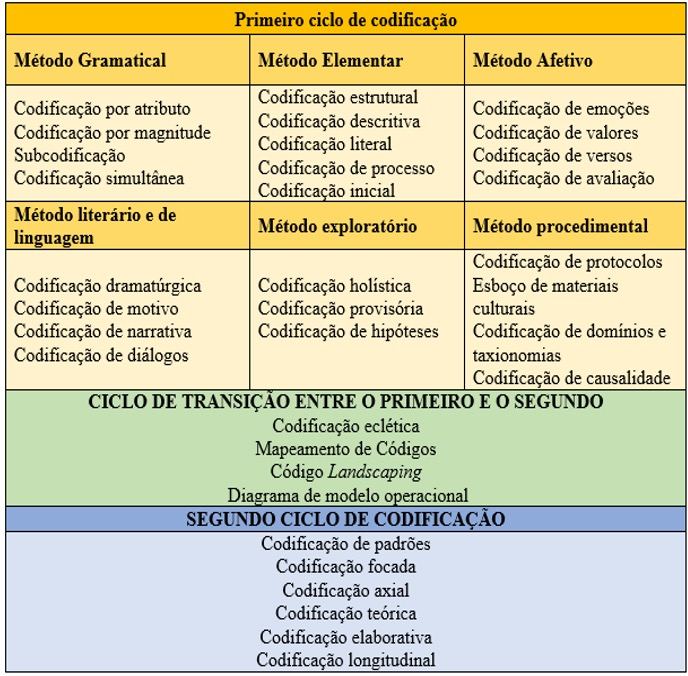
\includegraphics[width=\linewidth]{Fig1.png}
\caption{Ciclo de Codificação de Saldaña.}
\label{fig1}
\source{\cite{bley_ciclos_2019}}
\end{minipage}
\end{figure}

A análise resultou no agrupamento dos códigos em cinco grupos: A. Ações educacionais; B. Tipos de abordagem; C. Público-alvo; D. Ações de diversidade/STEAM; e E. Ações comerciais. Para elaborar a lista de categorias de cada grupo, foi realizado o Segundo Ciclo de Classificação, com o uso da Codificação de Padrões, definida por \textcite[p.~233]{saldana_coding_2013} como ``códigos explicativos ou inferenciais, que identificam um tema emergente, configuração ou explicação''. Entre o Primeiro e o Segundo Ciclo de Codificação, foi utilizado o Ciclo de Transição com a Codificação \textit{Landscaping} e a construção de uma nuvem de palavras no Atlas TI para identificar as categorias predominantes e possíveis subcategorias (\Cref{fig2}).

\begin{figure}[!htbp]
\centering
\begin{minipage}{0.75\textwidth}
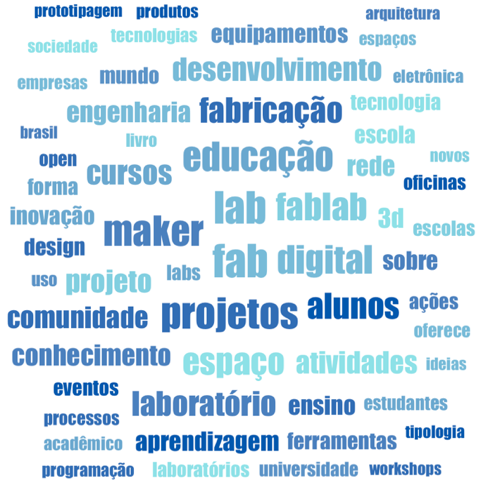
\includegraphics[width=\linewidth]{Fig2.png}
\caption{Nuvem de palavras do Ciclo de Transição de Saldaña.}
\label{fig2}
\source{Elaboração própria}
\end{minipage}
\end{figure}

A criação da nuvem de palavras no software Atlas TI serviu como norteador para o ajuste e agrupamento das categorias. Por exemplo, as palavras ``workshop'' e ``engenharias'' foram adicionadas após a construção da nuvem de palavras. Para \textcite[p.~199]{saldana_coding_2013}, o código Landscaping ``integra métodos textuais e visuais para ver tanto a floresta quanto as árvores. É baseado na técnica visual de ‘tags’, na qual a palavra ou frase mais frequente de um texto aparece maior do que as outras''.

Após a análise com os diferentes ciclos de codificação e refinamento das categorias, foi utilizado o processo de tematizar os dados indicado em \textcite[p.~175]{saldana_coding_2013} chegamos ao quadro final com os cinco grupos e suas 33 categorias (\Cref{tbl1}).

\begin{table}[h!]
\centering
\begin{footnotesize}
\caption{Grupos e categorias de análise.}
\label{tbl1}
\footnotesize
\begin{tabular}{>{\raggedright\arraybackslash}p{2.5cm} >{\raggedright\arraybackslash}p{2.5cm} >{\raggedright\arraybackslash}p{2.5cm} >{\raggedright\arraybackslash}p{2.5cm} >{\raggedright\arraybackslash}p{2.5cm}}
\toprule
A. Ações educacionais & B. Tipos de abordagem & C. Público-alvo & D. Ações de diversidade/STEAM & E. Ações comerciais \\ 
\midrule
A.1 Realização do Arduino Day/Scratch Day/Hachaton & B1. Aprendizagem criativa/cola\-bo\-ra\-ti\-va & C1. Ensino Fundamental & D1. Ações de diversidade étnico-racial & E1. Cobrança de serviços e parceiras pagas \\
A.2 Realização de eventos/festas/en\-con\-tros & B2. Educação investigativa &
C2. Ensino Médio & D2. Democratização do acesso às tecnologias & E.2 Consultoria e apoio para a implantação de espaços \textit{maker} \\
A.3 Foco em cursos/pa\-les\-tras/\textit{work\-shops} & B3. Educação Maker & C3. Ensino Superior/Cursos diversos & D3. Incentivo para as mulheres no uso de tecnologias & E.3 Marketing \\
A4. Foco na inovação e prototipagem com projetos & B4. Empreendedorismo & 
C4. Ensino Superior En\-ge\-nha\-rias/Design/Ar\-qui\-te\-tu\-ra/Com\-pu\-ta\-ção & D4. Incentivo ao STEAM & \\
A.5 Parceria com escolas sem custos & B5. Integração com a BNCC & C5. Estudantes da Comunidade & D5. Ações de sustentabilidade & \\
A.6 Parceria com centros de pesquisa & B6. Metodologias Ativas/PBL/Pro\-je\-tos
C6. Estudantes da Rede Pública & D6. Foco nas comunidades periféricas. & \\
A.7 Projeto de extensão de ensino superior & B7. Rede de compartilhamento & 
C7. Estudantes das Escolas Privadas. & & \\
A.8 Solução de problemas na Educação & B8. Uso do \textit{design thinking}. & & & \\
A.9 Formação de professores & & & & \\
\bottomrule
\end{tabular}
\source{Elaboração própria.}
\end{footnotesize}
\end{table}

Após a categorização no \textit{software} Atlas TI, foram elaboradas as redes semânticas que são uma representação gráfica dos dados analisados e possibilitam a visualização dos dados articulados com os recortes dos documentos e as categorias que foram atribuídas, como pode ser observado nas análises apresentadas no tópico a seguir.

\section{Análise e discussão dos resultados}\label{sec-fmt-manuscrito}
Iniciaremos a análise dos documentos dos 42 FAB LAB listados no site da \textit{FAB LAB Foundation} que indicavam em seus documentos alguma ação específica para a Educação. Apresentaremos primeiro a síntese da descrição de cada um (\Cref{tbl2}).

\begin{footnotesize}
\begin{longtable}{p{1cm} p{1cm} p{11.5cm}}
\caption{Descrição dos FAB LAB pesquisados.}
\label{tbl2}
\\
\toprule
FLAB1 & PE & O FLAB 1 tem uma ação chamada de maker school, na qual recebe alunos de escolas privadas para a realização de cursos e oficinas que são pagos. No dia do \textit{open day} realiza ações para as escolas públicas. Desenvolve atividades de consultoria na área de Educação Pública e privada por meio de convênio e acertos financeiros. Promove atividades de \textit{Hackathon, Arduino Day} etc. Tem vários projetos que podem ser aplicados em escolas com parcerias estabelecidas com o FAB LAB. \\
FLAB2 & RJ & O FLAB 2 tem ações direcionadas para o público periférico e pautadas nas ações afirmativas. Projetos Pretas, Aprenda com uma Avó, entre outros, têm foco nas minorias e na diversidade, entendendo que a democratização das tecnologias digitais é fundamental para garantir a equidade e o empoderamento desses grupos. \\
FLAB3 & SP & O FLAB 3 é voltado para a Educação Básica e para os cursos tecnológicos, com foco em projetos e aprendizagem criativa. É uma rede grande de FAB LAB distribuídos em várias das suas unidades com o nome de FAB LAB Escola. \\
FLAB4 & MG & O FLAB 4 é uma empresa que desenvolve soluções e oferece vários cursos que usam softwares específicos. O FAB LAB promove ações voltadas para a Educação Básica, especificamente as últimas séries do Ensino Fundamental e o Ensino Médio, por meio de competições intercolegiais. \\
FLAB5 & RJ & O FLAB 5 é um projeto de extensão que usa o espaço para a realização das atividades do Ensino Superior, usando a metodologia \textit{Design Thinking}. Faz referências aos objetivos sustentáveis do milênio e ao uso de atividades \textit{maker} nas disciplinas, mas não está indicado como isso acontece. \\
FLAB6 & AM & O FLAB 6 desenvolve atividades com crianças a partir de 6 anos, com foco na aprendizagem criativa e Educação \textit{Maker}. Aparentemente são oficinas/aulas/cursos para crianças das escolas privadas, com cobrança de mensalidades, mas isso não está claro no documento. \\
FLAB7 & MS & O FLAB Senai UEMS é um projeto de extensão com foco nos cursos de Engenharia e vários projetos de inovação. Criou um projeto de parceria com as escolas de ensino médio da rede pública para a realização de experimentos de Física. \\
FLAB8 & SC & O FLAB 8 fundamenta a sua proposta com elementos do movimento \textit{maker}, STEAM e as características da indústria 4.0. Isso é curioso porque o movimento \textit{maker} é um contraponto ao processo de industrialização, e não o seu reforço. O projeto tem uma proposta construtivista e está organizado em projetos de trabalho, com foco na Educação Básica. Apresenta a Educação Maker como uma solução pedagógica para os problemas de aprendizagem. \\
FLAB9 & SP & O FLAB 9 criou um ambiente que associa o uso das tecnologias digitais aos aspectos lúdicos (games, gincanas etc.) ou de lazer. O espaço pode ser usado para carregar o celular, descansar ou conhecer os projetos. Possui espaços de \textit{coworking} e oferece oficinas e cursos gratuitos e pagos. Os cursos ofertados têm o mesmo foco na prototipagem como os outros FAB LAB, com o acréscimo de oficinas sobre games, robótica e projetos temáticos (dia da gratidão, encontro de poliglotas, dia do astronauta etc.). \\
FLAB10 & RS & O FLAB 10 apresenta a estrutura de um projeto de extensão voltado para o desenvolvimento de seus alunos dos cursos de arquitetura, engenharia e computação. Realiza o \textit{open day} e tem ofertas de cursos voltados para a prototipagem. Realiza eventos, workshops e cursos, executando projetos de membros da comunidade externa. O FAB LAB só é aberto ao público externo uma vez por semana. \\
FLAB11 & SP & O FLAB 11 tem como proposta realizar ações que integrem as demandas de formação da indústria com o processo formativo dos alunos das escolas de Ensino Fundamental e Médio da rede. Realiza eventos e cursos e desenvolve parcerias sem custos. \\
FLAB 12 & MG & O FLAB 12 tem como proposta ser um centro de treinamento de pessoas e espaço de \textit{coworking} para o desenvolvimento de ações de \textit{startups} previamente selecionadas. Atende os cursos de engenharia da instituição e desenvolve alguns projetos para crianças e adolescentes em cursos pagos. Realiza eventos e o espaço fica aberto para a comunidade que pode integrar os projetos desenvolvidos no local. \\
FLAB13 & SP & O FLAB 13 é ligado à universidade tem como objetivo principal atender os alunos dos cursos de engenharia da instituição, mas também é aberto para a comunidade. As atividades são gratuitas para os membros da comunidade acadêmica e cobrados do público externo, dependendo do projeto. Oferece palestras, cursos e \textit{workshops}. \\
FLAB14 & MT & O FLAB 14 é vinculado ao Departamento de Arquitetura da universidade e realiza cursos para a comunidade interna e externa. Desenvolve projetos de pesquisa e execução de modelos e materiais para outros setores. \\
FLAB15 & PA & O FLAB 15 tem como proposta democratizar o acesso ao espaço maker e realiza cursos, \textit{workshops} e programas de incentivo às mulheres e meninas nas Ciências Exatas. \\
FLAB16 & PR & O FLAB 16 foi criado dentro de uma escola municipal e não possui todos os equipamentos de um FAB LAB para fazer parte da rede mundial de FAB LAB, indicando uma falha no processo de cadastramento no site do FAB LAB Foundation. Atende os alunos da escola, todos no Ensino Fundamental, e permite o uso do público externo. \\
FLAB17 & PB & O FLAB 17 é um espaço acadêmico vinculado à universidade e foi criado inicialmente para desenvolver materiais didáticos e metodologias inovadoras para os alunos dos cursos de Engenharia, Design e Arquitetura. Oferece cursos para a comunidade interna e externa. \\
FLAB18 & SC & O FLAB 18 é classificado como acadêmico e está vinculado à universidade. Voltado para os cursos de Engenharia, Design e Arquitetura, também oferece cursos para a comunidade externa, mas o seu foco é a prototipagem e a execução de projetos para os cursos. \\
FLAB19 & SP & O FLAB 19 está vinculado à uma universidade privada e atende cursos diversos. Também oferece cursos para o Ensino Fundamental e Médio. Usa a proposta como marketing da instituição. \\
FLAB20 & SP & O FLAB 20 é apresentando como a primeira rede de FAB LAB voltado para a Educação Básica. Está integrado a uma rede de escolas da Educação Básica. \\
FLAB21 & SP & O FLAB 21 é direcionado para os cursos de Engenharia e Arquitetura e tem uma proposta comercial de aluguel de equipamentos e do espaço, assim como a cobrança de cursos. Na abertura do site, a primeira informação é sobre o pagamento dos serviços com o uso de cartão de crédito na reserva. \\
FLAB22 & MA & O FLAB 22 é fruto de um convênio entre uma empresa de mineração e o governo do Maranhão, para atender as escolas em seu laboratório \textit{maker} e com visitas aos espaços escolares, levando os equipamentos. \\
FLAB23 & SP & O FLAB 23 é voltado para os cursos de Engenharia, com foco na prototipagem. Não oferece cursos e usa o FAB LAB como marketing da instituição. \\
FLAB24 & SC & O FLAB 24 tem como proposta um trabalho social e trabalha exclusivamente com voluntários. Aluga o seu espaço para empresas e instituições de ensino. \\
FLAB25 & CE & O FLAB 25 é voltado para crianças. Faz cobrança de serviços e oferece cursos e palestras para a comunidade. \\
FLAB26 & RS & O FLAB 26 é totalmente voltado para o público acadêmico e tem como foco a prototipagem e execução de projetos dos cursos de Engenharia. Não trabalha de forma colaborativa e não disponibiliza o \textit{open day}, obrigatório para fazer parte da FAB LAB Foundation. \\
FLAB27 & SP & O FLAB 27 tem como proposta a democratização no acesso ao uso de tecnologias digitais com abordagem \textit{maker}, oferecendo cursos e apoio ao desenvolvimento de projetos. Desenvolve uma ação interessante de residência \textit{maker} para formação em projetos abertos e \textit{maker}. \\
FLAB28 & RN & O FLAB 28 está dentro de uma escola privada, vinculado à Startup Maker Educ, que oferece serviços para a implantação de ações \textit{maker} nas escolas, com foco nas crianças. \\
FLAB29 & SP & O FLAB 29 está localizado dentro de uma instituição de nível superior e tem como proposta apoiar os cursos de Engenharia, Administração e Design na construção de projetos e prototipagem. Usa o FAB LAB como ação de \textit{maketing}. \\
FLAB30 & MG & O FLAB 30 está vinculado ao centro universitário e serve como apoio para os cursos da instituição. Realiza cursos e \textit{workshops} e indica preocupação com o compartilhamento de projetos. Atende a comunidade no \textit{open day}. \\
FLAB31 & CE & O FLAB 31 está localizado dentro do parque tecnológico e vinculado à Universidade Federal Atende alunos de diversos cursos e empresas. Oferece cursos e \textit{workshops} que são pagos. \\
FLAB32 & RS & O FLAB 32 é um projeto de extensão universitária e tem como foco os cursos de Computação. Oferece cursos e tem atendimento aberto à comunidade, sem custos. Desenvolve ações com a Educação Básica e com o Ensino Superior. \\
FLAB33 & SP & O FLAB 33 tem como foco a Educação Básica e desenvolve várias ações com foco na robótica. Promove eventos dentro dos movimentos mundiais e oferece cursos para a comunidade. \\
FLAB34 & SP & O FLAB 34 funciona dentro de um shopping e pertence a uma Instituição de Ensino Superior. Oferece cursos pagos e gratuitos e usa o espaço como estratégia de \textit{marketing}. \\
FLAB35 & PI & O FLAB 35 é vinculado à Universidade Federal. Foi criado para atender ao curso de Arquitetura, mas ampliou as suas ações para atender a comunidade. É um espaço acadêmico e desenvolve algumas ações educacionais, tendo como um dos focos a Educação Maker. Tem foco também na cultura, desenvolvendo projetos de artistas e eventos culturais. \\
FLAB36 & SE & O FLAB 36 é vinculado a uma instituição privada de Ensino Superior e tem como objetivo atender os alunos. Abre o espaço para a comunidade duas vezes por semana. \\
FLAB37 & RS & O FLAB 37 desenvolve atividades para os alunos de Design e Arquitetura. Abre o espaço para a comunidade três vezes por semana, oferece cursos e \textit{workshops} e faz parcerias com escolas da rede pública, sem custo. \\
FLAB38 & MG & O FLAB 38 atende os cursos da instituição de diversas áreas, tem foco na prototipagem e inovação e abre o espaço para a comunidade uma vez por semana. \\
FLAB39 & RS & O FLAB 39 atende a comunidade acadêmica, com foco nos cursos de Engenharia, Arquitetura e Design. Abre o espaço uma vez por semana para a comunidade e desenvolve parcerias com empresas privadas. \\
FLAB40 & SP & O FLAB 40 é um laboratório privado que faz menção ao trabalho educativo, mas o foco é na produção e apoio para o artesanato. Tem um \textit{open day} uma vez por semana aberto para a comunidade. \\
FLAB41 & SC & O FLAB 41 é um espaço de ensino, pesquisa e extensão da universidade, coordenado pelo curso de Design, com foco nas áreas de Design, Arquitetura, Engenharias, Artes e afins. Faz parte de uma rede de laboratórios localizados em diferentes cidades da região e oferece apoio aos alunos de graduação e pós-graduação, aos professores, com consultoria e cursos em diferentes áreas. \\
FLAB42 & SP & O FLAB 42 é o primeiro FAB LAB independente do país. É um espaço de ensino, pesquisa e extensão na área da materialização da forma por meio de técnicas automatizadas. \\
\bottomrule
\source{Elaboração própria.}
\end{longtable}
\end{footnotesize}

A síntese da descrição de cada FAB LAB serviu como uma referência para encontrarmos os elementos convergentes nos dados e nas análises, mas também apontou divergências significativas nos documentos, como veremos a seguir.

\subsection{Ações educacionais do FAB LAB}\label{sec-formato}
O primeiro grupo de análise é o grupo A. Ações Educacionais, com nove categorias. Os resultados indicam o predomínio de duas ações: a realização de cursos, palestras e \textit{workshops}, seguido do foco na execução de projetos de inovação e prototipagem. A realização de cursos surge vinculada à perspectiva de disseminação da cultura \textit{maker}, formação de pessoas e adesão ao movimento \textit{maker} para a fabricação, como podemos ver no recorte a seguir:

\begin{quote}
    Nossos cursos e oficinas atendem os mais diversos públicos. Com o incentivo à inovação, criatividade e estímulo às ideias materializadas através da fabricação digital e interação com a rede mundial Fab Lab, a unidade oferece cursos incríveis (Documento do FAB LAB 35).
\end{quote}

As menores ocorrências foram parcerias com escolas sem custos, formação de professores e solução de problemas na Educação. É interessante observar que justamente as categorias mais relacionadas com a Educação foram as menos mencionadas nos documentos, mas isso também pode ser resultado da concepção de ação educacional que esses espaços têm. Nos espaços em que a formação de professores foi mencionada, identificamos uma preocupação com o processo de apropriação da cultura \textit{maker} \Cref{fig3}.

\begin{figure}[htbp]
\centering
\begin{minipage}{\textwidth}
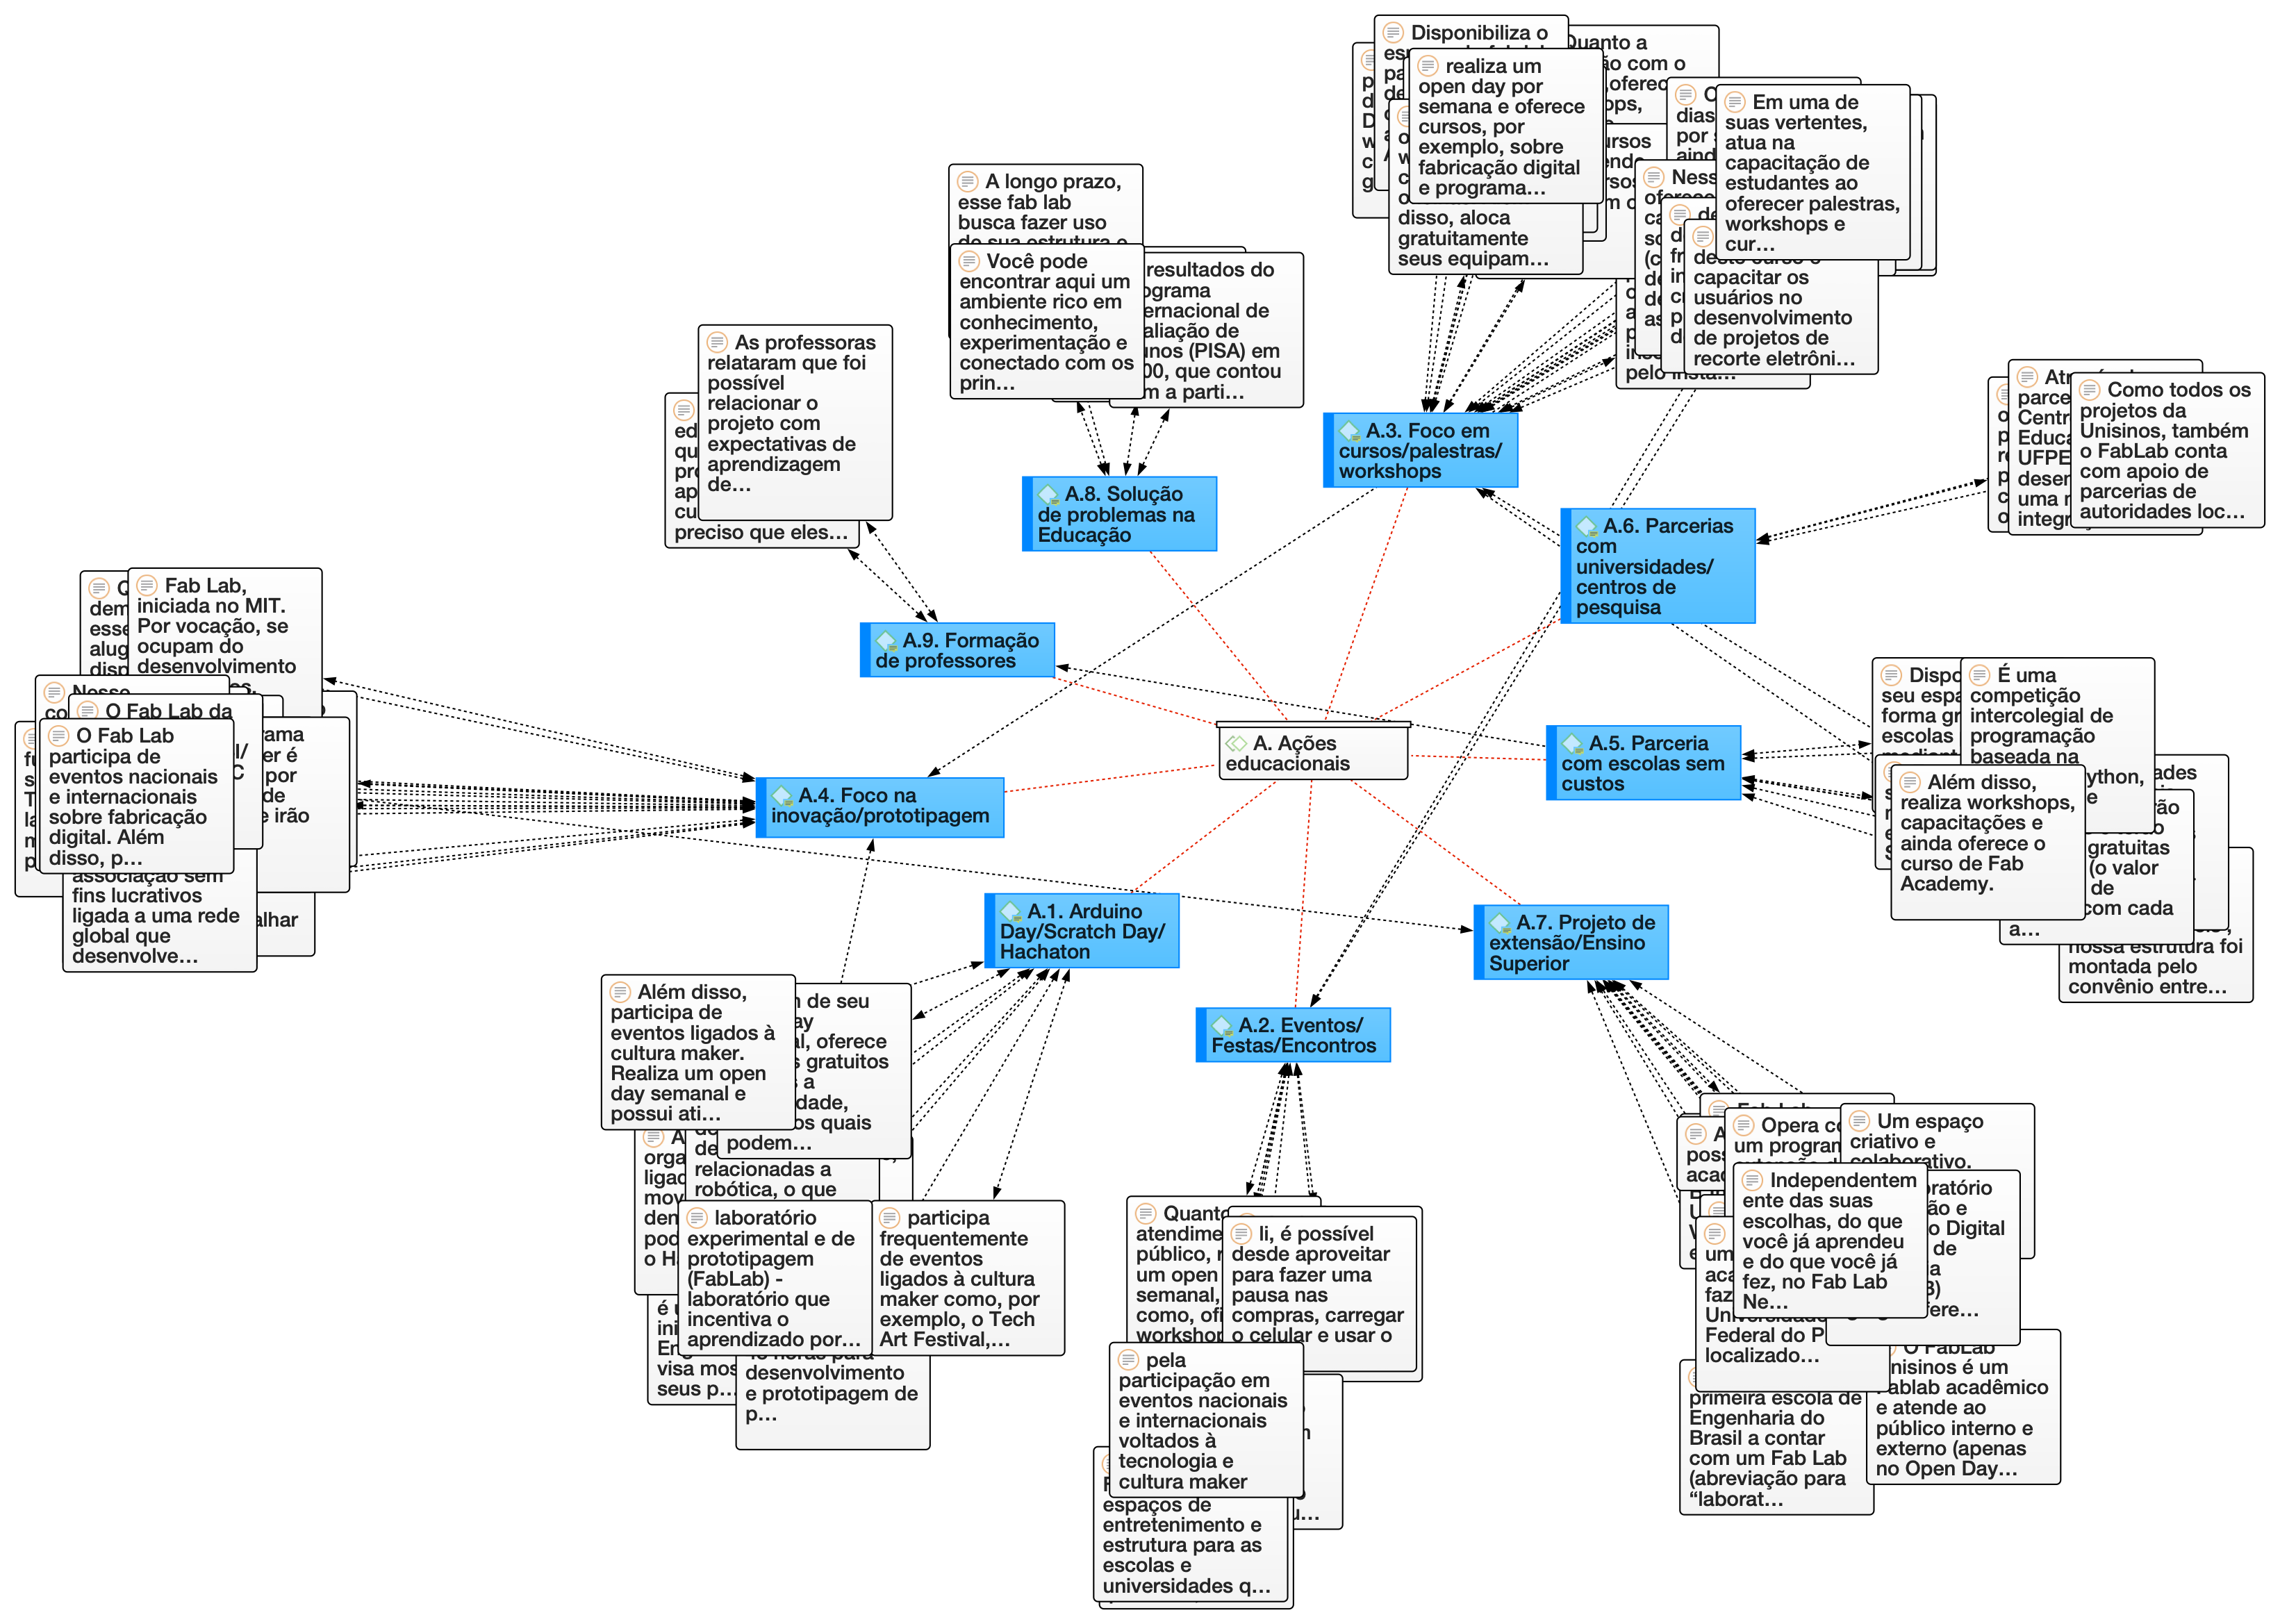
\includegraphics[width=\linewidth]{Fig3.png}
\caption{Rede de ações educacionais.}
\label{fig3}
\source{Elaboração própria.}
\end{minipage}
\end{figure}

A oferta de cursos está associada ao maquinário existente nos laboratórios \textit{maker}, mas poucos indicaram a formação de professores em suas ações, mesmo os laboratórios localizados dentro de instituições de ensino. O apoio aos projetos de prototipagem é considerado como foco principal em vários documentos institucionais, como podemos verificar no recorte a seguir:

\begin{quote}
    O laboratório está equipado com recursos qualificados de fabricação digital para dar suporte à pesquisa básica e ao desenvolvimento de novos produtos, processos e serviços. O foco do Laboratório concentra-se no uso da prototipagem nas fases iniciais de projetos inovadores (Documento do FAB LAB 28).
\end{quote}

Na categoria solução para os problemas da Educação, encontramos alguns recortes interessantes nos documentos:

\begin{quote}
    Verificou-se que estes alunos do curso desenvolviam poucas atividades práticas e poucas atividades de extensão junto à comunidade. Preocupado com isso, decidiu-se promover essas ações junto com os alunos para que os mesmos pudessem potencializar seus conhecimentos e habilidades em Engenharia, além de promover uma mudança social, pois localmente as escolas públicas não possuem estrutura nem profissionais qualificados para desenvolverem as ações que aproximem os alunos destes temas mais tecnológicos e inovadores (Documento do FAB LAB 8).
\end{quote}

No recorte, há uma referência ao uso da cultura \textit{maker} como um elemento que pode suprir as deficiências da Educação, associada à ideia de modernidade ou inovação.

\subsection{Tipo de abordagem do FAB LAB}\label{sec-modelo}
No grupo B. Tipo de abordagem, foram selecionadas oito categorias. Nesse grupo as categorias emergiram dos documentos e foi possível encontrar a combinação de duas ou mais categorias no mesmo laboratório. Nos resultados encontrados, predominou a proposta de Educação Maker e, em seguida, o empreendedorismo (\Cref{fig4}).

\begin{figure}[htbp]
\centering
\begin{minipage}{\textwidth}
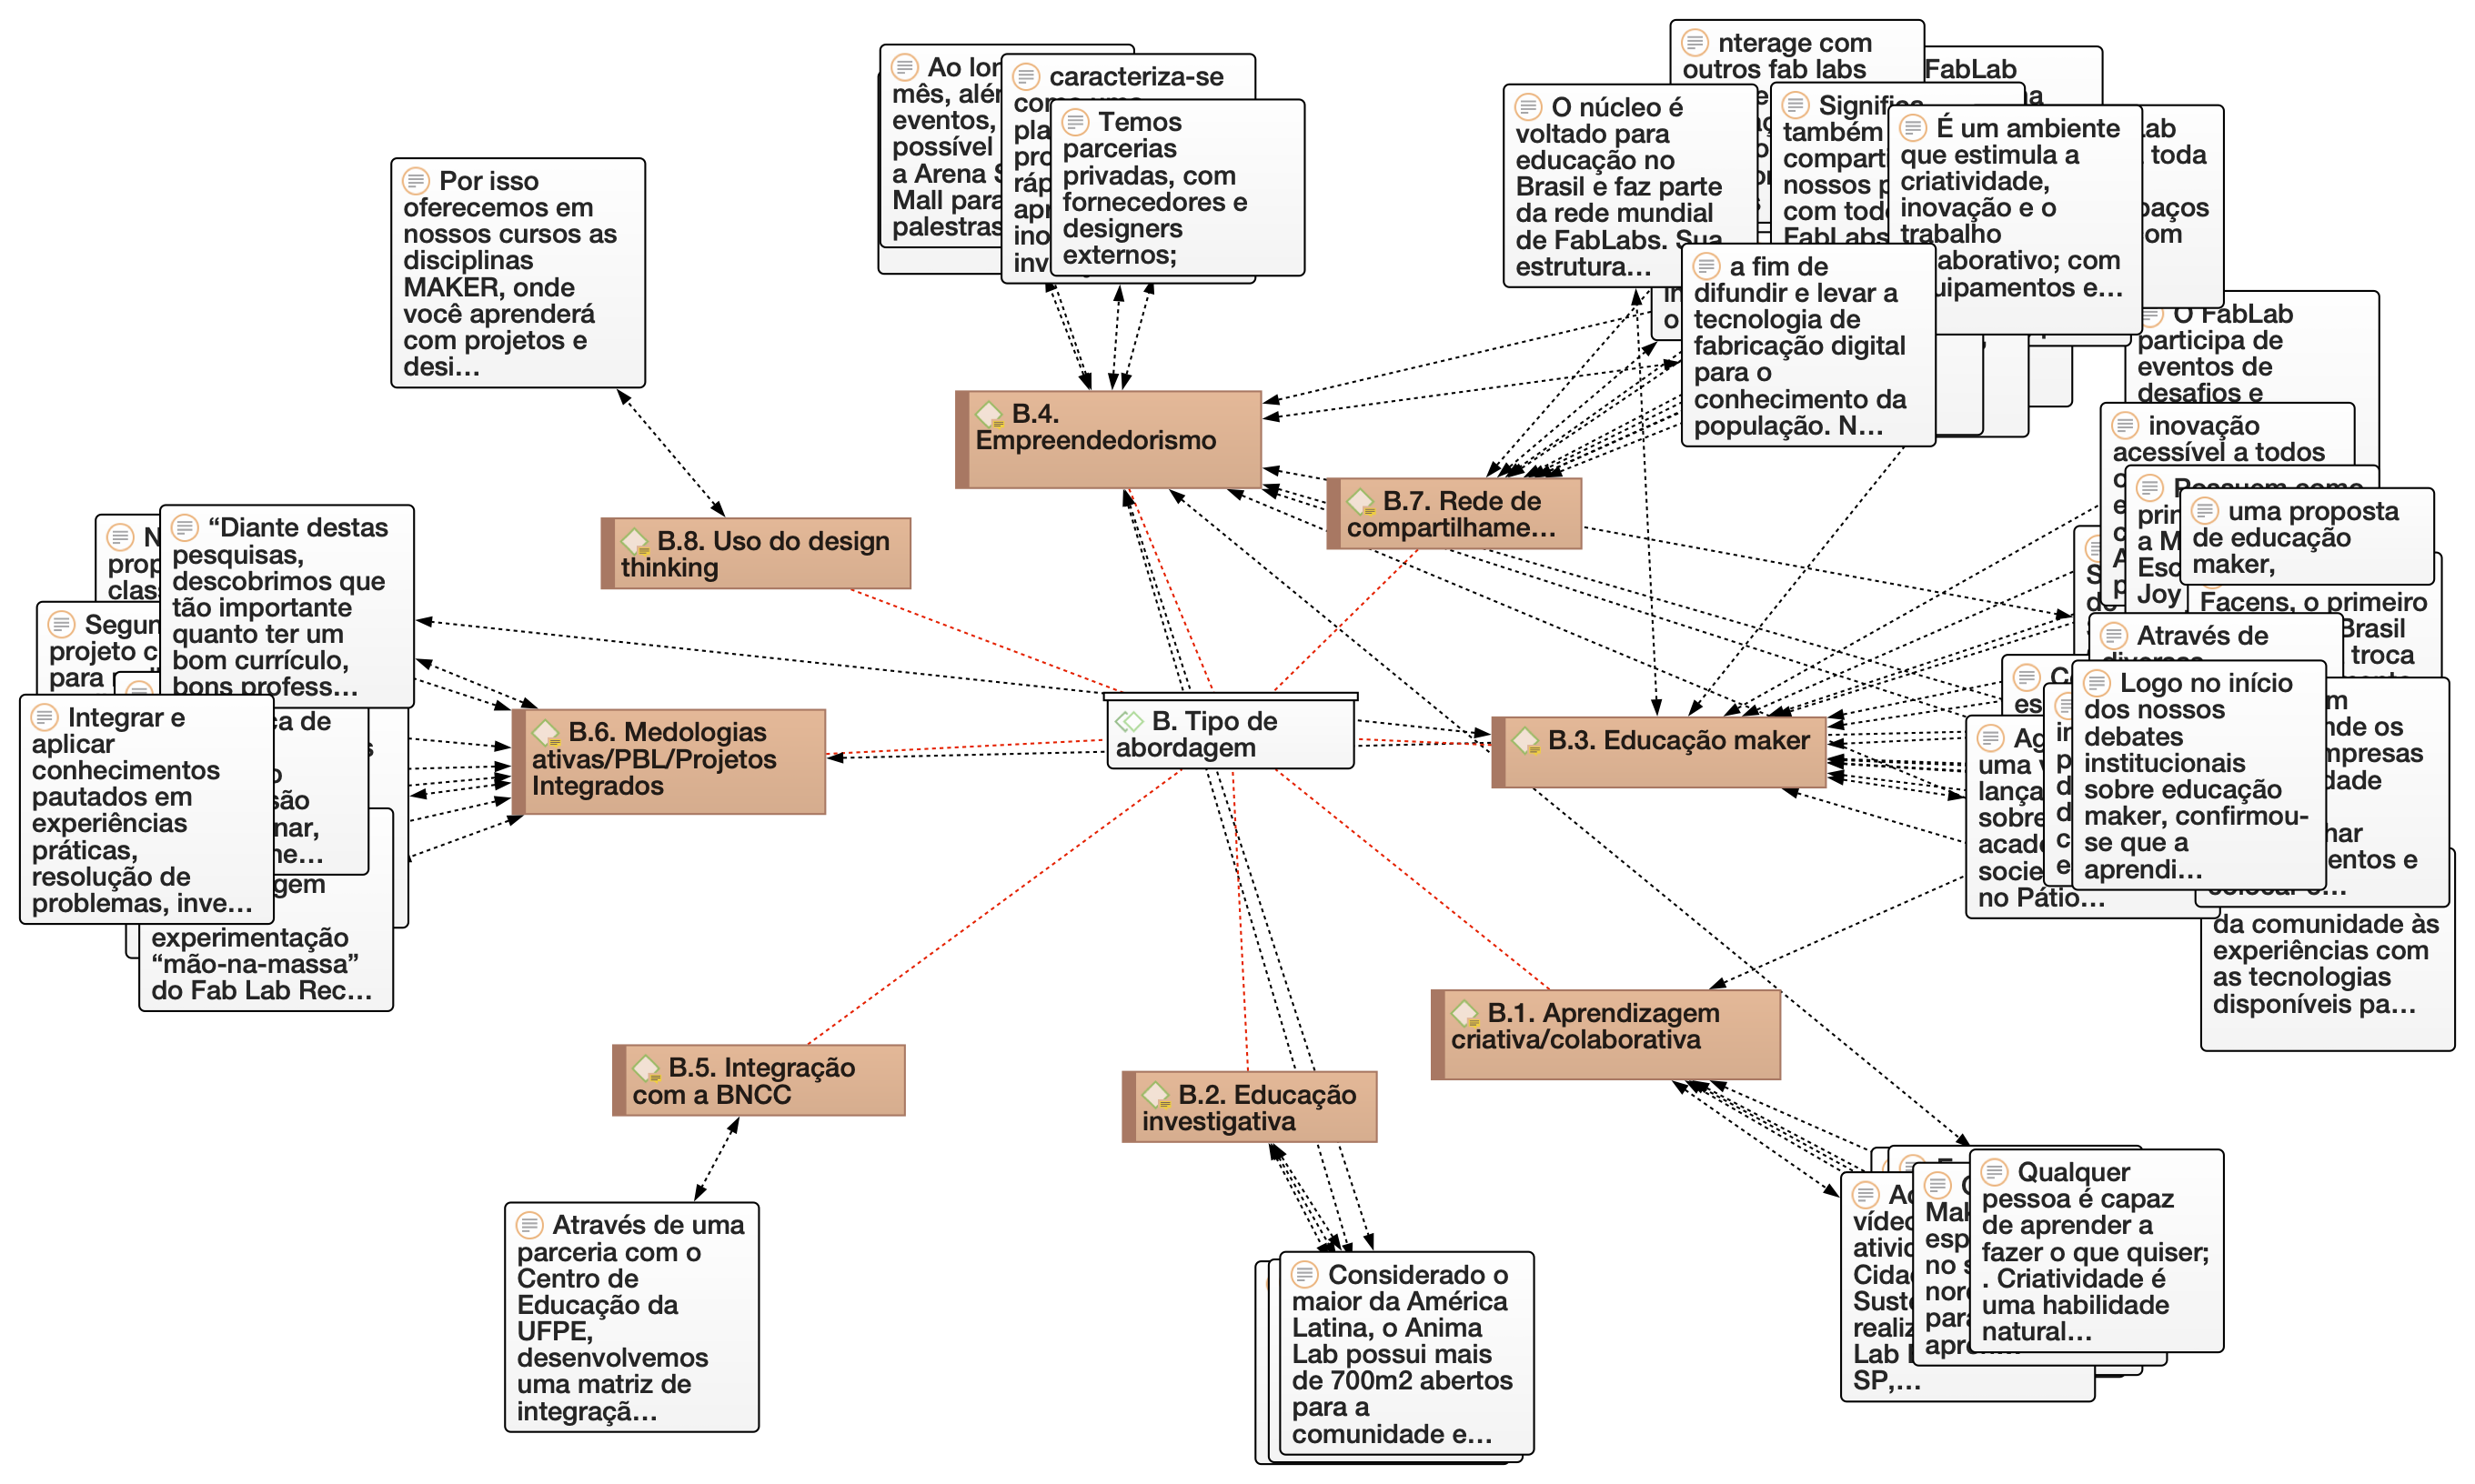
\includegraphics[width=\linewidth]{Fig4.png}
\caption{Tipo de abordagem do FAB LAB.}
\label{fig4}
\source{Elaboração própria.}
\end{minipage}
\end{figure}

É importante ressaltar que a Educação Maker foi associada aos elementos mão na massa, como aprender fazendo, construção, experiências, compartilhamento, empreendedorismo e inovação, como podemos verificar nos recortes das citações encontradas no documento a seguir:

\begin{quote}
    Concomitante a esse cenário, na contemporaneidade, cada vez mais, as relações sociais e, em especial, o mundo do trabalho, exigem um sujeito/profissional que tenha, além da excelência técnica, aptidões como liderança, empreendedorismo, criatividade, trabalho em equipe, entre outras habilidades que são fundamentais para a realidade (Documento do FAB LAB 19).
\end{quote}

O empreendedorismo surge com duas vertentes nos documentos: invenção e produção como uma possibilidade de negócios ou oportunidade de melhoria econômica e social para pessoas de comunidades periféricas. As abordagens relacionadas com aprendizagem criativa, metodologias ativas e projetos correspondem a menos da metade das propostas, resultado realmente surpreendente, considerando os objetivos apontados em todos os documentos.

\begin{quote}
    Diante destas pesquisas, descobrimos que tão importante quanto ter um bom currículo, bons professores-mentores, tecnologias disponíveis, precisávamos mudar também as metodologias de aprendizagem e, claro, os espaços disponíveis. O Lab, assim, nada mais é que um grande espaço de aprendizagem, uma ``sala de aula'' ampliada e diferenciada (Documento do FAB LAB 13).
\end{quote}

A categoria Rede de compartilhamento ou a necessidade de compartilhar projetos e soluções só foi mencionada, de forma explícita ou implícita, em 6 documentos, como no recorte a seguir:

\begin{quote}
    Os projetos estão disponíveis no repositório e organizados em temas (saúde, design, robótica, mobiliário, jogos e brinquedos educativos, equipamentos mecatrônicos, máquina de fabricação digital, instrumentos musicais, games, software livre, arquitetura e urbanismo, artes cênicas, acessibilidade, dispositivos mecânicos, dispositivos eletrônicos, sustentabilidade e transporte) (Documento do FAB LAB 29).
\end{quote}

Os princípios da rede mundial de FAB LAB consideram a colaboração e o compartilhamento como essenciais para que o espaço faça parte da rede, mas da mesma forma que encontramos FAB LAB afirmando não realizar o \textit{open day} e ``compensando'' com outras ações, temos também espaços que não indicam a necessidade de compartilhamento de projeto com os usuários.

\subsection{Público-alvo do FAB LAB}\label{sec-organizacao}
O grupo C. Público-alvo apresenta sete categorias e os resultados são interessantes: metade dos laboratórios desenvolve ações para o público do Ensino Fundamental e Médio e a outra metade para os alunos do Ensino Superior (\Cref{fig5}). Poucos desenvolvem ações para os dois públicos e, quando isso acontece, as ações estão relacionadas com o perfil da instituição vinculada ao FAB LAB.

\begin{figure}[htbp]
\centering
\begin{minipage}{\textwidth}
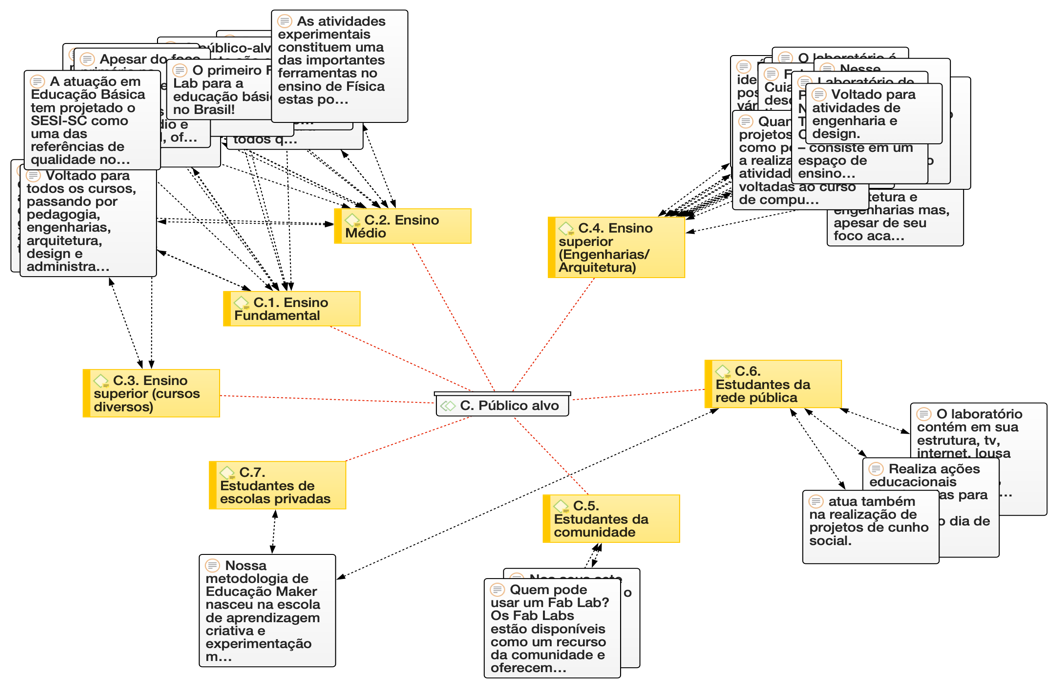
\includegraphics[width=\linewidth]{Fig5.png}
\caption{Público-alvo do FAB LAB.}
\label{fig5}
\source{Elaboração própria.}
\end{minipage}
\end{figure}

O Ensino Superior foi dividido em Ensino Superior (Cursos Diversos) e Ensino Superior (Engenharias, Design, Arquitetura e Computação). Isso foi necessário porque detectamos um desequilíbrio entre os cursos que são atendidos por ações do FAB LAB: o número de laboratórios com foco nos cursos diversos é muito inferior ao número dos que realizam ações para cursos específicos de Engenharia, Computação etc.

Os documentos assumem claramente o foco com o seu público-alvo, como podemos verificar na citação a seguir:

\begin{quote}
    Utilizado principalmente por alunos de Design, Arquitetura e Engenharias mas, apesar de seu foco acadêmico, é um espaço aberto à comunidade (Documento do FAB LAB 14).
\end{quote}

Apenas dois FAB LAB realizaram ações com foco nos dois níveis (Educação Básica e Ensino Superior). As ações destinadas ao atendimento específico para alunos da rede pública, privada ou da comunidade, foram categorias que emergiram dos documentos e encontradas em poucos FAB LAB.

\subsection{Ações de diversidade e incentivo ao STEAM do FAB LAB}\label{sec-organizacao-latex}
Em relação ao agrupamento D. Ações de diversidade e incentivo STEAM, encontramos seis categorias e nos resultados, prevaleceram as ações relacionadas com a democratização das tecnologias (\Cref{fig6}).

\begin{figure}[htbp]
\centering
\begin{minipage}{\textwidth}
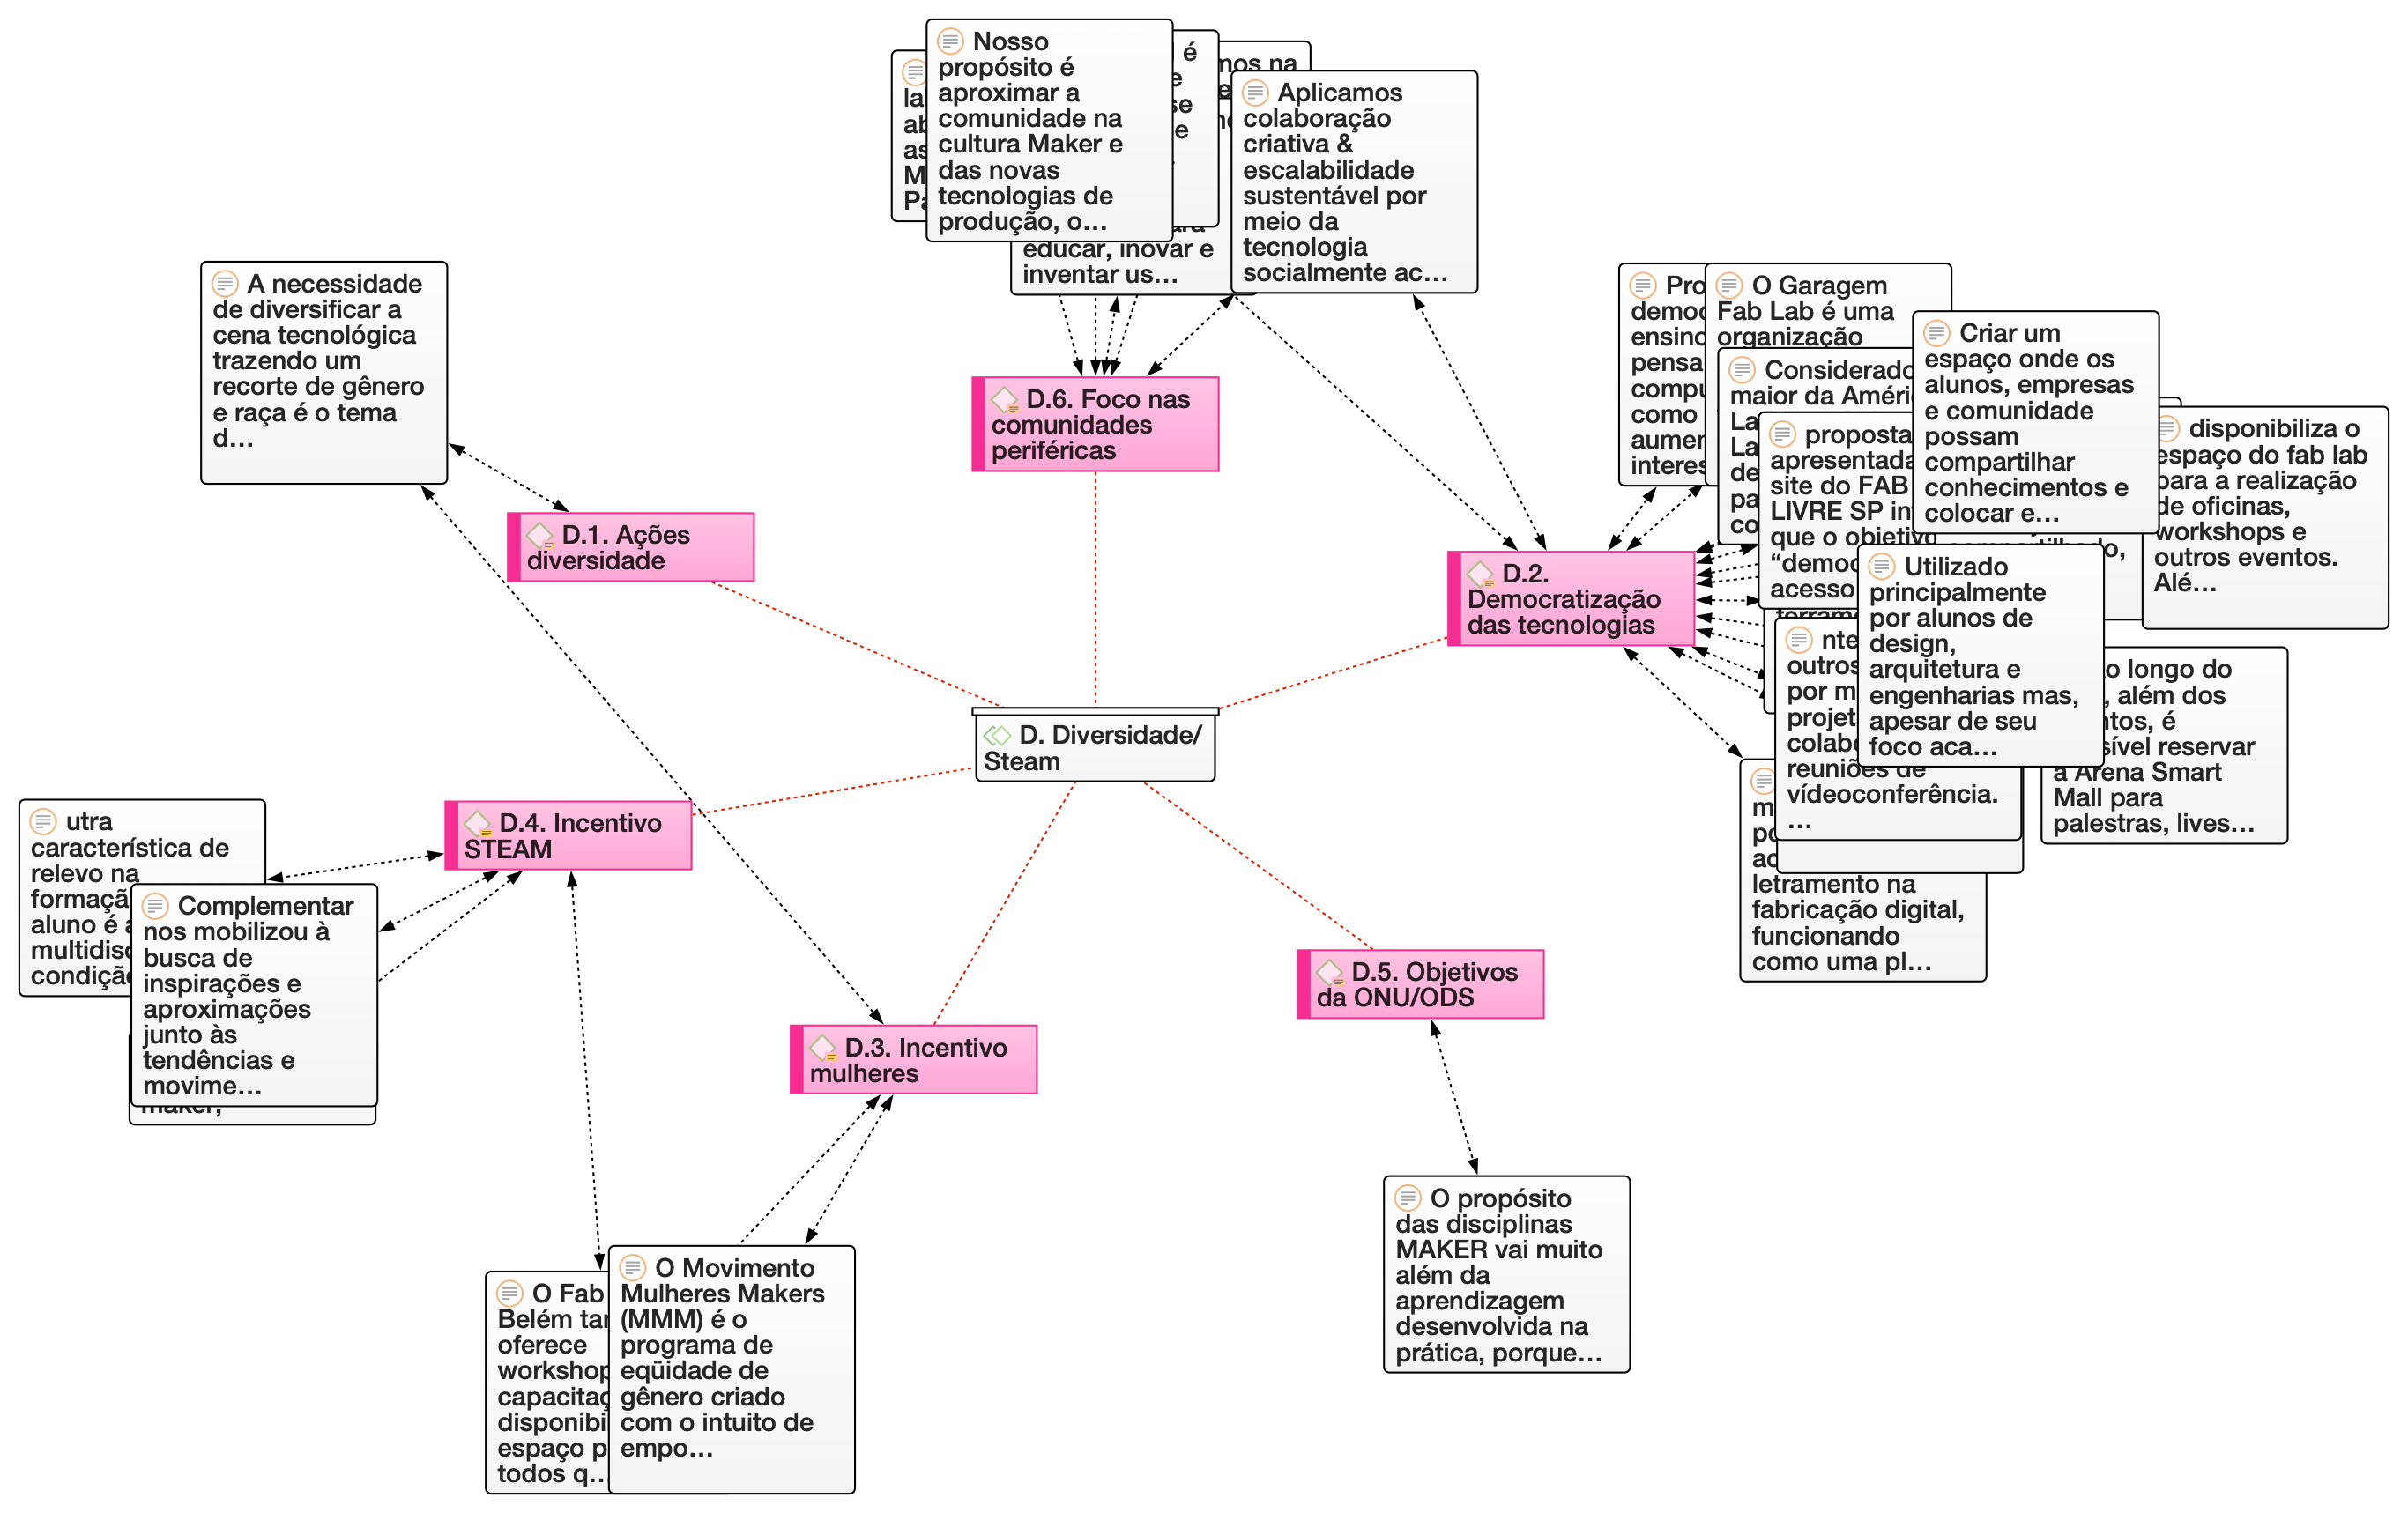
\includegraphics[width=\linewidth]{Fig6.png}
\caption{Ações de diversidade e incentivo ao STEAM do FAB LAB.}
\label{fig6}
\source{Elaboração própria.}
\end{minipage}
\end{figure}

A citação a seguir demonstra a proposta de democratização existente nesses espaços.

\begin{quote}
    O LAB é uma organização social que surgiu com o objetivo de fomentar a criatividade, a democratização da tecnologia e o desenvolvimento de projetos apoiados na filosofia do ``Faça Você Mesmo'' (Documento do FAB LAB 23).
\end{quote}

As ações de diversidade apareceram em apenas dois Fab Labs. O texto relacionado com a questão étnico-racial é bem contundente:

\begin{quote}
    Defendemos a diversidade como um valor fundamental a ser incorporado em nossa cultura, pois acreditamos que todos devem ter direito às mesmas oportunidades e que o racismo estrutural e a desigualdade social que marcam o nosso país precisam ser severamente combatidos. Só assim conseguiremos criar um país melhor para todos e que aproveita a potência criativa da sua população (Documento do FAB LAB 2).
\end{quote}

As ações de incentivo para as mulheres foram indicadas em três FAB LAB, com projetos específicos, e um dos espaços (FLAB2) que realiza essa ação também realiza ações afirmativas com foco na diversidade, como mostram a citação a seguir:

\begin{quote}
    A necessidade de diversificar a cena tecnológica trazendo um recorte de gênero e raça é o tema deste projeto, que nasceu em 2017 como uma rede de mulheres negras na tecnologia e hoje possui um braço de formação educacional e outro de consultoria de diversidade para empresas (Documento do FAB LAB 2).
\end{quote}

O incentivo ao STEAM foi identificado em apenas 4 laboratórios, o que é contraditório com o número de espaços que priorizam os cursos da área de Exatas. É possível que as ações propostas com eventos, cursos e palestras oferecidos sejam compreendidas como movimentos de incentivo ao STEAM, mas não é possível ignorar a enorme desigualdade de oportunidades econômicas e de gênero que existe no país e até mesmo em países europeus.

Em relação à existência de ações relacionadas com a sustentabilidade, apenas um documento indicou essa possibilidade com o seguinte argumento:

\begin{quote}
    Aplicamos colaboração criativa \& escalabilidade sustentável por meio da tecnologia socialmente acessível de forma a promover economia de abundância e assim gerar soluções locais e globais (Documento do FAB LAB 16).
\end{quote}

As ações direcionadas especificamente para as comunidades periféricas foram encontradas em cinco laboratórios, como se vê abaixo:

\begin{quote}
    Acreditamos na potência que as periferias do mundo têm para apontar caminhos e soluções. Acreditamos também que boas ideias surgem de cidadãos comuns, empenhados em construir novos mundos. Por isso, ouvimos o que os grandes fóruns e os espaços mais relevantes de discussão global apontam como tendências, mas estamos sempre de olho nas ideias e pensamentos que emergem de maneira descentralizada, nos lugares mais improváveis (Documento do FAB LAB 2).
\end{quote}

Mais uma vez, o FAB LAB 2 indicou realizar atividades específicas para as comunidades periféricas, além de desenvolver projetos de ações afirmativas e de incentivo para as mulheres.

\subsection{Ações comerciais no FAB LAB}\label{sec-titulo}
O último agrupamento analisado foi o E. Ações comerciais, com três categorias. Consideramos que esse agrupamento aborda um tema sensível, sobretudo porque existem regras claras sobre os princípios dos FAB LAB e nem todos os espaços pesquisados seguem esses princípios. As ações comerciais categorizadas envolvem objetivos diferentes e predominou a cobrança de serviços ou parcerias pagas e, em seguida, as ações de marketing para divulgar o próprio FAB LAB ou outros negócios vinculados (\Cref{fig7}).

\begin{figure}[htbp]
\centering
\begin{minipage}{\textwidth}
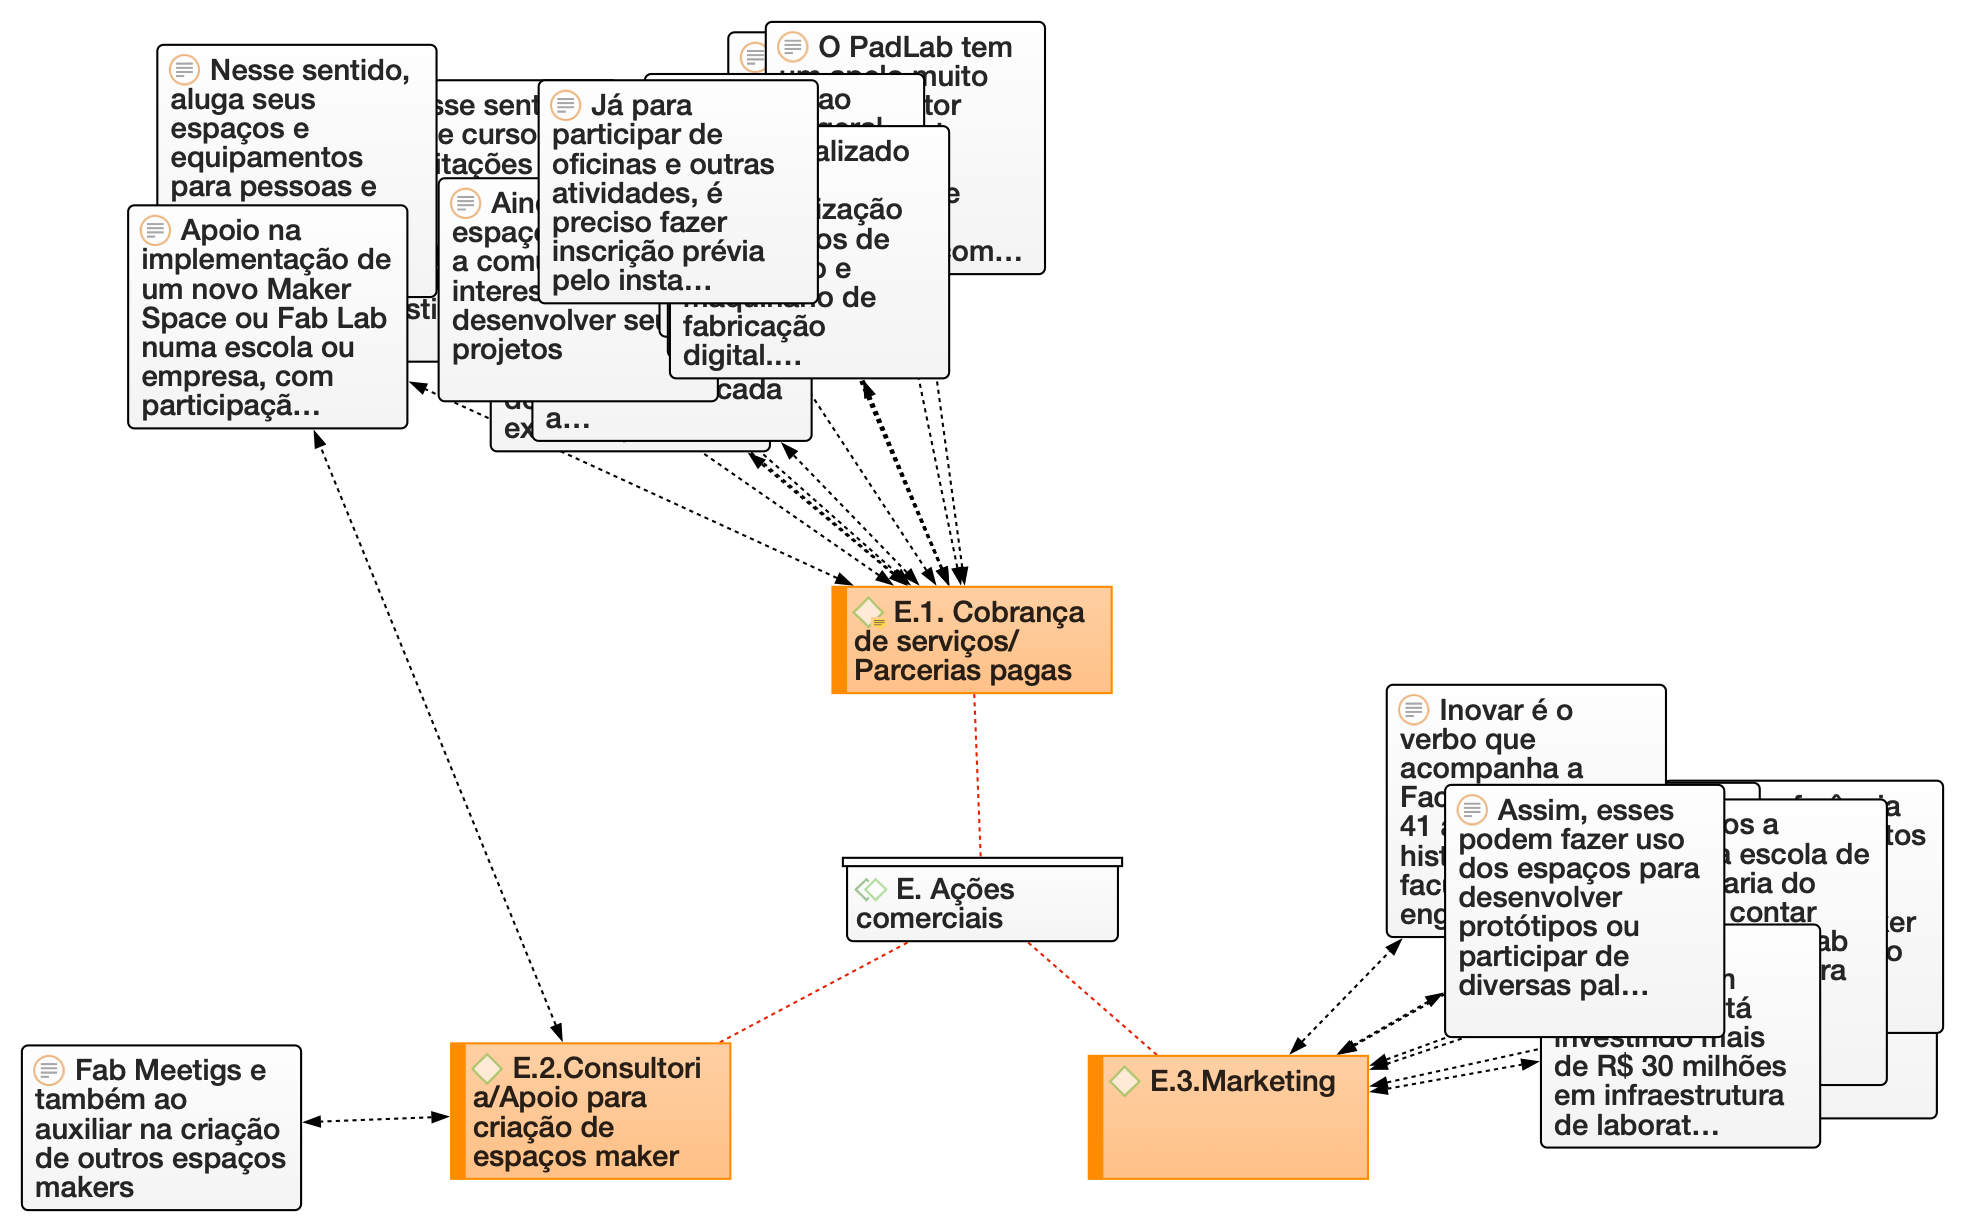
\includegraphics[width=\linewidth]{Fig7.png}
\caption{Ações comerciais no FAB LAB.}
\label{fig7}
\source{Elaboração própria.}
\end{minipage}
\end{figure}

Foram encontrados 13 laboratórios indicando a cobrança de serviços ou parcerias pagas e 7 instituições que utilizam o FAB LAB como estratégia de \textit{marketing}, associando o laboratório ao ensino de qualidade, inovação, modernidade, metodologias ativas etc., como podemos identificar nas citações a seguir:

\begin{quote}
    Inovar é o verbo que acompanha a nossa instituição. Em seus 41 anos de história, as Faculdades de Engenharia, Tecnologia e Arquitetura e Urbanismo já foram muitas vezes pioneiras e tiveram muitas iniciativas inéditas e disruptivas (Documento do FAB LAB 36).
\end{quote}

É importante observar que, mesmo quando havia indicação de algum tipo de contrapartida financeira, só consideramos a existência de cobrança de serviços quando estava explícito no documento do Fab Lab, como no exemplo a seguir:

\begin{quote}
    Caso você não possua cartão de crédito para realizar o pagamento no ato da reserva, você deve inserir créditos em sua conta antes de fazer a reserva, fazendo pagamento na tesouraria e entregando pessoalmente uma via do comprovante para um dos colaboradores do Fab Lab. Assim iremos inserir crédito na sua conta manualmente (Documento do FAB LAB 22).
\end{quote}

As ações relacionadas com consultorias e apoio para a criação de espaços \textit{maker} foram indicadas em apenas dois FAB LAB. A cobrança de serviço que foi indicada nos documentos inclui a oferta de cursos, aluguel de espaço, uso de equipamentos, eventos e palestras. Os serviços são oferecidos para pessoas individualmente, empresas, escolas e órgãos públicos.

É importante ressaltar que a cobrança de serviços predomina nos espaços de instituições privadas, embora algumas instituições públicas cobrem por alguns serviços específicos. A ausência do \textit{open day}, uma das exigências para ter associação com a FAB LAB Foundation, é um dado importante, porque indica que algumas instituições não cumprem as orientações, mesmo estando vinculadas e listadas na página oficial dos FAB LAB como podemos ver no recorte a seguir:

\begin{quote}
    Disponibiliza o espaço do FAB LAB para a realização de projetos pela comunidade acadêmica. Assim, por mais que não realize open day, oferece minicursos gratuitos, por exemplo, sobre impressão 3D, assim como workshops, dentre os quais se destaca o de arquitetura algorítmica''. (Documento do FAB LAB 36)
\end{quote}

A possibilidade de uma instituição registrada no site internacional da FAB LAB Foundation indicar nos seus documentos oficiais que não segue um dos princípios mais importantes estabelecido para garantir a inserção na lista, indica que existe uma dificuldade no acompanhamento e controle dos espaços que se apresentam como integrantes da rede de FAB LAB mundial.


\section{Conclusão}\label{sec-idioma}
A cultura \textit{maker} no campo da Educação está em processo de construção e em movimento constante. O que conseguimos captar nesta pesquisa é um recorte do momento, que certamente sofrerá muitas transformações nos próximos anos e isso é muito positivo. Os resultados indicam que poucos FAB LAB atuam no campo da Educação, mas, quando isso acontece, os resultados são muito positivos. Os resultados da análise dos documentos indicam que a pouca atuação dos FAB LAB na Educação pode ser resultado também da compreensão equivocada sobre os processos formativos. A oferta de cursos ou o foco nos projetos de prototipagem não são elementos suficientes para disseminar a cultura \textit{maker} nos espaços formais de Educação, porque se materializam como ações pontuais e não integradas ao currículo.

Como apontado nas pesquisas de \textcite{blikstein_educacao_2020,soster_educacao_2020}, existe uma grande diversidade de abordagens e práticas da cultura \textit{maker}, o que indica que ainda temos um caminho a percorrer para a compreensão e consolidação dos princípios do movimento \textit{maker} e suas possíveis aplicações na Educação. O mosaico de teorias de aprendizagem e o uso de abordagens diversas, em alguns casos até conflitantes, podem fragilizar e até mesmo neutralizar os benefícios produzidos com as ações \textit{maker}.

No Ensino Superior, o foco exclusivamente em cursos que, por sua natureza, já têm afinidades com a prototipagem, como Engenharias, Design e Arquitetura, embora tenham como proposta transformar as metodologias de aprendizagem nesses cursos, não avançam em outras áreas do conhecimento dentro dos espaços acadêmicos. Esse resultado confirma o que foi apontado no relatório de \textcite{vossoughi_making_2015}, no qual os autores afirmam que ``others are examining if and how making can support student engagement in the scientific and engineering practices elucidated in the recent Framework for K12 Science Education'' \textcite[p.~4]{vossoughi_making_2015}.

A cultura \textit{maker} é muito ampla e disruptiva para ficar restrita a uma área do conhecimento. Por outro lado, o incentivo para os alunos do Ensino Médio se interessarem pela área STEAM, foco dos FAB LAB vinculados ao Ensino Superior, foi encontrado em pouquíssimos espaços.

Um aspecto bastante preocupante que os resultados indicaram é a ausência de ações que contemplem a diversidade e que tenham foco nas necessidades das minorias. Os princípios do manifesto \textit{maker} que serve como referência para a rede FAB LAB mundial promovem o compartilhamento, colaboração e integração de todos, mas vários FAB LAB não seguem esses princípios e poucos vão além com a realização de ações com foco na diversidade.

A existência de alguns FAB LAB ou propostas de espaço \textit{maker} comprometidos com a disseminação e consolidação da cultura \textit{maker} na Educação mostra que é possível articular ações efetivas com excelentes resultados. Embora o \textit{maker} ainda esteja muito associado aos equipamentos e às habilidades para o seu uso, existem outros elementos que precisam ser tratados com igual importância. Eles estão relacionados com a concepção de uso desses espaços e as diretrizes para a disseminação dos princípios \textit{maker}, que precisam se propagar para além dos laboratórios e alcançar outros espaços, até mesmo os mais inesperados.


\printbibliography\label{sec-bib}
%conceptualization,datacuration,formalanalysis,funding,investigation,methodology,projadm,resources,software,supervision,validation,visualization,writing,review

\end{document}
